%! TEX root = thesis.tex
% vim: ft=tex et sts=2 sw=2

\chapter{Introduction}

This thesis is a potpourri of some results that span everything from classical mechanics, to statistical mechanics, to quantum mechanics, to engineering.
A common thread that connects these fields is that of asymptotics and geometry.

\begin{figure}
  \begin{center}
    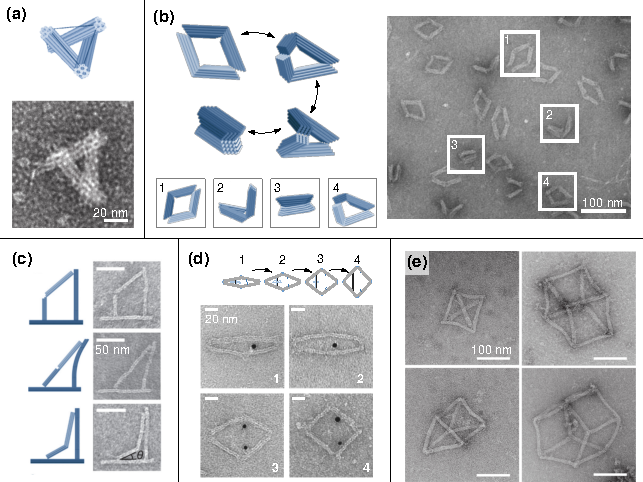
\includegraphics{dna.pdf}
  \end{center}
  \caption{DNA origami has been widely used to self assemble a variety of objects at the nanoscale.
    Depicted in the figure are (a) tensegrity structures \cite{liedl2010}; (b), (c) linkage-based mechanisms \cite{marras2015,zhou2015}; (d) a rhombus-shaped nanoactuator~\cite{ke2016}; and (e) self-assembled polyhedra~\cite{iinuma2014}.  All images used with permission.}
  \label{fig:dna_origami}
\end{figure}

\begin{figure}
  \begin{center}
    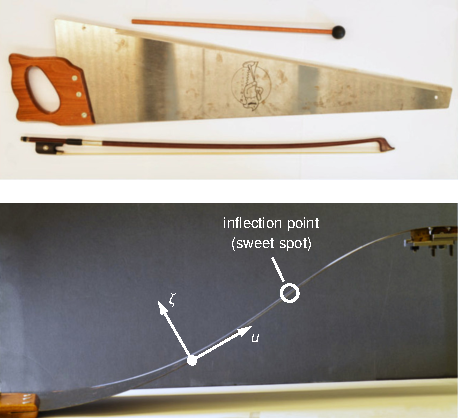
\includegraphics{saw/saw.pdf}
  \end{center}
  \caption{%
    An ordinary wood saw when bent into the shape of an S can be played like a musical instrument using a violin bow or a mallet.
    A sustained note is produced on bowing or hitting the saw at its inflection point, which is called a sweet spot by musicians.
    Photographs adapted from Ref.~\cite{shankar2022} and used with permission.
  }
  \label{fig:saw}
\end{figure}

\section{Organizational summary}

This dissertation is organized as follows:
Finally, in Appendix~\ref{app:math}, we collect some helpful mathematical results that are used throughout the dissertation.
